To calculate the fully-coherent mismatch, we will model the random walk as a
zero-mean Gaussian walk in the phase, frequency, and spin-down which occurs at
$\Nsd$ fixed time intervals, $\Delta T$ such that the total observation time is
$\Tobs = \Nsd \Delta T$.
This allows us to write the signal as 
a piecewise Taylor expansion with $N$ subdomans. Choosing fixed time intervals appears to
introduce an additional timescale not usually present in random walk models.
However, as discussed in Appendix~\ref{sec: physical interpretation of the monthly
ephemeris} this is consistent with a large number of unresolved events which
are measured over a fixed timescale.

In this model, the spin-down rate will be the highest order term which
undergoes a random walk. Recalling that $\Delta \dot{f}_i$ (defined in
Eqn.~\eqref{eqn: Delta Phi}) is the difference between the signal and template
in the $i^{th}$ subdomain, we may define the jump in this difference between
the $i$ and $i-1$ subdomains as $\tn \fdot_i$, such that
\begin{equation}
\Delta \fdot_{i} - \Delta\fdot_{i-1} = \tn \fdot_{i} \sim \mathcal{N}(0, \sigS),
\end{equation}
where $\mathcal{N}$ denotes the normal distribution and we have defined $\sigS$
as the standard-deviation of the step sizes in the spin-down rate. The residual
between parameter space offsets is denoted by $\tn$ which is normally
distributed. Rearranging this gives an expression for the offset in the
$i^{th}$ subdomain, by induction we can also write down the $i-1$ term
\begin{align}
\Delta\fdot_{i} &  = \tn\fdot_{i} + \Delta\fdot_{i-1}  \\
\Delta\fdot_{i-1} &  = \tn\fdot_{i-1} + \Delta\fdot_{i-2}  .
\end{align}
Let us set the initial difference between the signal and template as zero such
that $\Delta\dot{f}_0=0$, that is we start each random walk from the origin
(we will return to this point in Section~\ref{sec: Random walk models part
II}). Then as each step proceeds from the previous step, we have that
\begin{equation} 
\Delta\fdot_{i} = \s{j=1}{i}\tn\fdot_{j}.
\label{eqn: delta fdot n} 
\end{equation}

To illustrate this, in Figure~\ref{fig: Illustration fdot int} we plot an example
of a random walk in spin-down as given by Eqn.~\eqref{eqn: delta fdot n}.
\begin{figure}[ht]
\centering
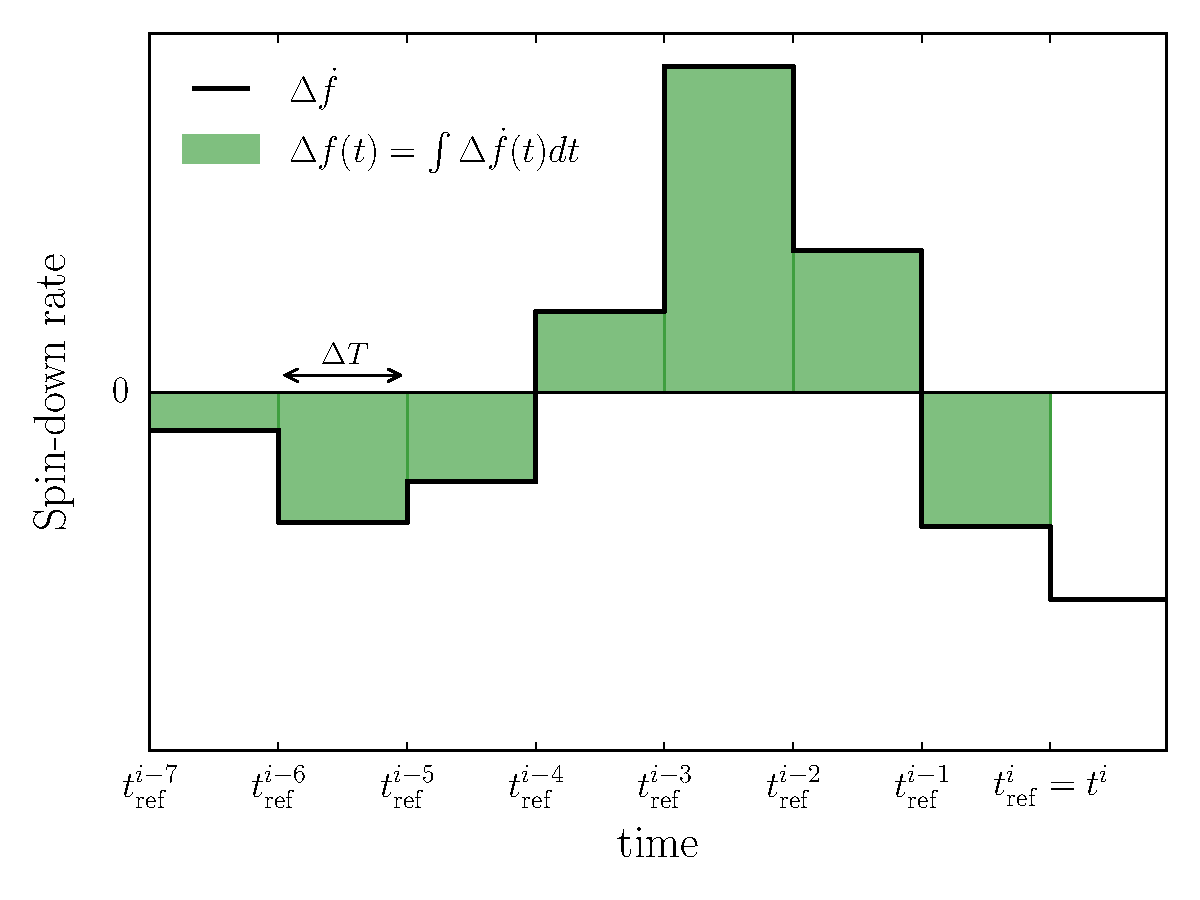
\includegraphics[width=0.7\textwidth]{Illustration_F1_int}
\caption{An example of a random walk in the spin-down rate, 
Eqn.~\eqref{eqn: delta fdot n}. The filled green blocks indicate the
summation defined in Eqn.~\eqref{eqn: f offset induced} required to
calculate the induced change in frequency at $t^{i}$ due to the random walk in
spin-down rate.}
\label{fig: Illustration fdot int}
\end{figure}

If we want to model a random walk in the phase, frequency, and spin-down rate
concurrently, then we must consider the effect that a
random walk in spin-down will have on the frequency and phase. For example, if we
increase the spin-down rate for a period of time, then we would expect the frequency
to decrease at a greater rate during this period. In our discreet model, it is
not possible to dynamically change the frequency during a single subdomain.
However, we can approximate this by updating the frequency in the next
subdomain with the induced frequency offset due to the spin-down in previous
subdomains. This must be done for the induced effect from the random walk in spin-down rate on
the phase and frequency, and for the induced effect from the random walk in frequency
on the phase. There is induced effect for the spin-down rate: the effect only
propagates to lower order terms.

Because the random walk is discreet and constant in any given subdomain, we can
calculate the offset in the lower order terms from a Taylor expansion. The
total offset at the  $i^{th}$ reference time is then given by the summation of
the offset caused by all higher order terms up to that reference time. The
reference times can be arbitrarily chosen, but setting each to start at the
beginning of the subdomain simplifies the calculation. 
The frequency offset induced by the spin-down can be
calculated using a Taylor expansion
\begin{equation}
\Delta \f_{i} = \s{j=1}{i-1}\Delta\fdot_{j} \dT .
\label{eqn: f offset induced} 
\end{equation}
This can be though of as the integration of the spin-down up to the $i^{th}$
reference time and is illustrated by the green blocks in Figure~\ref{fig:
Illustration fdot int}. 

Since we want to consider random walks in all three parameters we now add in a
random walk in frequency. Each step is independent of the induced effect from
the spin-down and is given by \mbox{$\tn \f_{i} \sim \mathcal{N}(0, \sigF)$}. The two
effects will sum linearly such that the frequency offset is
\begin{equation}
\Delta \f_{i} = \s{j=1}{i}\tn \f_{j} + \s{j=1}{i-1}\Delta\fdot_{j} \dT.
\label{eqn: f offset} 
\end{equation}

By a similar process we can calculate the induced effect of the frequency and
spin-down on the phase. Including the random walk in the phase
for which $\delta \phi_i \sim \mathcal{N}(0, \sigP)$, the phase offset is given by
\begin{equation}
\Delta\phi_{i}  =  \s{j=1}{i}\tn \phi_{j} 
+ 2\pi\left(\s{j=1}{i-1}\Delta \f_{j}\dT 
+ \frac{1}{2}\s{j=1}{i-1}\Delta \fdot_{j}\dT^{2}\right).
\label{eqn: phi offset}
\end{equation}

%Equations \eqref{eqn: f offset} and \eqref{eqn: phi offset} will allows us to
%construct the parameter space offsets in all three terms from the distibutions
%$\tn \phi_i$, $\tn \phi_i$, and $\tn \phi_i$.


